\newpage
\section{Ütemezési algoritmusok}

Az ütemezési feladat megfogalmazható mint:
\[
\begin{rcases}
J_i \mbox{ -- munkák} \\
P_i \mbox{ -- megmunkálási idő} \\
w_i \mbox{ -- súly} \\
d_i \mbox{ -- határidő} \\
r_i \mbox{ -- rendelkezésre álló idő} \\
C_i \mbox{ -- befejezési iödő} \\
\end{rcases}
\Rightarrow 
\parbox[t]{9cm}{ $+$ egy adott időben egy gépen egy munka folyik \\
és létezik egy célfügvény amire nézve optimális ütemezést keresünk.}
\]

Egy halmazfeladat gyors leírására a következő struktúrát használjuk:
\[
\underbrace{\alpha}_{\mbox{gépi infó}} | \underbrace{\beta}_{\mbox{ütemezési infó}
} | \underbrace{\gamma}_{\mbox{optimalizálási kritérium}}
\]

\begin{description}
  \item[gépi információ] alatt a rendelkezésre álló gép számosságot értjük. Lehet:
  \begin{itemize}
  \item $1$ -- egy gép áll rendelkezésre.
  \item $P_m$ -- $m$ darab párhuzamosan futó gép
  \item $P$ -- a párhuzamosan futó gépek száma nincs rögzítve, tartalmazza az $1,2,\cdots$ feladatokat is.
\end{itemize}
  \item[ütemezési információ] azt mondja meg, hogy milyen ütemezést illető
  megkötéseink vannak a halmaz elemeire:
  \begin{itemize}
  \item \emph{prec} -- létezik egy irányított a--ciklikus gráf amely
  meghatározza, hogy a munka elkezdéséhez mely munkák kellet már befejeződjenek.
  \item $r_j$ -- egy--egy munkának tudjuk, hogy mely időponttól áll rendelkezésünkre.
  \item $P_j$ -- tudjuk, hogy egy--egy munka elvégzése mennyi időt vesz igénybe
  (ez mindig adott).
\end{itemize}
  \item[optimalizálási kritérium] arra vonatkozik, hogy a célfüggvényben mire
  fektetünk hangsúlyt:
  \begin{itemize}
  \item $C_{\mbox{max}}=\mbox{max}(C_j)$ -- utolsó munka befejezési ideje legyen minél
  kisebb (gyorsan befejezni a csomagot).
  \item $\sum C_j = \sum \frac{C_j}{n}$ -- a munka átlagos befejezési ideje
  legyen a lehető legkisebb (átlagosan keveset várjunk a gépekre).
\end{itemize}
\end{description} 

\subsection{ \texorpdfstring {$ 1||C_{max} $} {1||Cmax} }

Egy gépre teljes átfutási idő szerint optimizálunk. $C_{\mbox{max}}=\sum_{i=1}^{n}
P_i \Rightarrow$ tehát csak felrakjuk a munkákat sorba, ügyelve arra, hogy ne 
létezzen pillanat amikor a gép áll és optimális megoldást kapunk.

\subsection{ \texorpdfstring {$ 1|prec|C_{max} $} {1|prec|Cmax} }

Most olyan sorrendben végezzük el a felrakást, hogy ne legyen munka amire a
függőség még nem fejeződőt be. Ez a sorrend egy irányított a--ciklikus gráfban
(DAG) nem mást mint a topologikus sorrend. Tehát első pontnak vegyünk egy forrás
pontot a precedencia gráfból, ezt töröljük és ismételjük e folyamatot amíg
létezik pont a gráfban. Ez polinomiális időben optimális megoldást ad.

\subsubsection{Topologikus sorrend meghatározása}

Adjunk hozzá a bemeneti DAG--hoz egy extra $s$ élet amelyet a végén törölni
fogunk. Minden $s \mapsto v, v \in V$ élt rakjuk be a gráfba. Minden pontra két
címkét vezessünk: az egyik azt mutatja, hogy a pont elért e, és ha igen mely
csúcsból; a másik érték meg azt jelzi, hogy a csúcs átvizsgált már e vagy sem.
Kezdetben $s$ elért, de nem átvizsgált.

Amig létezik elért, de még nem átvizsgált él addig ismételjük: 

\begin{itemize}
  \item kiválaszt a legkésőbb elért de nem átvizsgált pontot $\mapsto u$
  \item ha létezik $u \mapsto v$ él a gráfban, ahol $v$ nem elért legyen $v$
  cimkéje elért $u$--ból.
  \item ha nem talál akkor $u$ címkéje lesz átvizsgált, feljegyezve, hogy az 
  algoritmus éppen hányadik lépésnél tart.
\end{itemize}

Az átvizsgálási sorrend lesz a topologikus sorrend, ha $s$ nem tagja az eredeti
gráfnak töröljük azt. Ha megfelelő adatstruktúrát használunk mindez az élszámmal
arányos időt vesz igénybe. Példa feladat:


\[
\begin{rcases}
G(V,E) &\mbox{összefüggő gráf} \\
c:E \mapsto \mathbb{R}^+ &\mbox{költségfüggvény} \\
V = \{ &T\mbox{--beli terminálok}, \\
	   &S\mbox{--beli Steiner pontok}\}
\end{rcases}
\parbox[L]{7cm}{ Keressünk minimális költségű fát $G$--ben, ami az összes
terminált tartalmazza és esetleg pár Steiner pontot is.} \]

Ha $T=V$ (tehát a gráfban nem léteznek Steiner pontok) akkor a feladat mohó
algoritmussal megoldható, egyébként meg NP--nehéz. A metrikus Steiner fában
a költségfüggvény kielégíti a háromszög egyenlőtlenséget:


\[ \parbox[l]{4cm}{
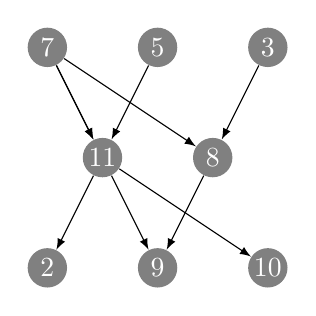
\begin{tikzpicture}[scale=0.7]
  \tikzset{ p/.style={circle,white,fill=gray,inner sep=0pt,minimum size=0.5cm},
  }
  \node[p] (7) at (-2, 2) {$7$};
  \node[p] (5) at (0, 2) {$5$};
  \node[p] (3) at (2, 2) {$3$};
  \node[p] (11) at (-1, 0) {$11$};
  \node[p] (8) at (1, 0) {$8$};
  \node[p] (2) at (-2, -2) {$2$};
  \node[p] (9) at (0, -2) {$9$};
  \node[p] (10) at (2, -2) {$10$};
  
  % the connection between the dots
  \draw[-latex] (7) -- (11) node [midway, above] {};
  \draw[-latex] (7) -- (8) node [midway, above] {};
  \draw[-latex] (5) -- (11) node [midway, above] {};
  \draw[-latex] (3) -- (8) node [midway, above] {};
  \draw[-latex] (7) -- (11) node [midway, above] {};
  \draw[-latex] (11) -- (2) node [midway, above] {};
  \draw[-latex] (11) -- (9) node [midway, above] {};
  \draw[-latex] (11) -- (10) node [midway, above] {};
  \draw[-latex] (8) -- (9) node [midway, above] {};
\end{tikzpicture}}
\parbox[l]{10cm}{
Az itt látható gráfnak több topologikus rendezése is van:

\begin{itemize}
  \item $7,~5,~3,~11,~8,~2,~10,~9$
  \item $7,~5,~11,~2,~3,~10,~8,~9$
  \item $3,~7,~8,~5,~11,~10,~9,~2$
  \item $3,~5,~7,~11,~10,~2,~8,~9$
\end{itemize}
}\]

\subsection{ \texorpdfstring {$ 1||\sum C_j$} {1||SumCj} }

\begin{description}
  \item[Shortest--Processing--Time -- SPT] minél rövidebb egy munka annál korábban
  rakjuk fel.
\end{description}

\emph{A Shortest--Processing--Time optimális megoldást ad a feladatra.}
\vspace{0.4cm}

A bizonyításhoz, tegyük fel, hogy az SPT nem ad optimális megoldást. Legyen
$p_1, p_2, \cdots, p_n$ egy optimális megoldás, ami nem SPT típusú. Tehát
létezik $p_i>p_{i+1}$ (szomszédos elemek). 

Látszik, hogy az összegen ekkor csak $C_i$ és $C_{i+1}$ változik meg. Tehát a
felcserélés végre hajtásával a $\sum C_j$ csökken, de ez ellentmondás a
feltevésünknek, tehát az SPT optimális.

\subsection{ \texorpdfstring {$ P_2||C_max$} {P2||Cmax} }

Ez egy NP--nehéz feladatt mivel visszavezethető a partíció problémára. Legyen
$a_1, a_2, \cdots, a_n \in \mathbb{Z}^*$. A kérdés, hogy létezik e $I \subseteq
\{1,2, \cdots, n \}$ amire $\sum_{i \in I} a_i = \sum_{i \not \in I} a_i$. Ez
meg a részösszeg speciális esete. Vegyük most a megmunkálási időket $\{p_1$, $p_2$,
$\cdots$, $p_n\}$, ekkor, ha OPT$=\frac{\sum P_i}{2} \Leftrightarrow$ létezik $p$
szám sorozatnak jó partíció. 

Tehát nem létezik hatékony algoritmus a feladatra, ezért a problémának speciális
eseteit és approximációs megoldásokat vizsgálunk meg.

\subsection{ \texorpdfstring {$ P||\sum C_j$} {P||Cmax} }

\begin{description}
  \item[List Scheduling -- LS -- listás ütemezés] Legyen $k$ gép és
  $P_{i=\overline{1,n}}$ feladat. Rakjuk fel ezeket sorrendben a gépekre, ha
  valamely gép végez megkapja a listában a következő munkát.
\end{description}

Ez egy elég primitív módszer hiszen gyakorlatilag csak arra ügyelünk, hogy a
gépeink ne álljanak. Ennek ellenére, ha $m$ gép van  az LS egy $2 - \frac{1}{m}$
approximációt ad. Ennek belátásához legyen $C^*_{\mbox{max}}$ az optimális
ütemezés. Erre fent állnak a következő alsó becslések:

\[ \frac{\sum P_i}{m} \leq C^*_{\mbox{max}} ~~~\mbox{ és }~~~
   P_{k \in i} \leq \mbox{max} (P_i) \leq C^*_{\mbox{max}}. 
\]

Most legyen $J_k$ az a munka melyet az LS ütemezés utoljára befejez. Ez egy $t$
pillanatban kezdődik el és tart $P_k$ idő intervallumot ($t+p_k=C_{\mbox{max}}$).
E adott $t$ időpontig az összes gép dolgozik, megállás nélkül, mert, ha ez nem
így lenne stratégiánk szerint a $P_k$ feladatott az a gép kapná meg. Tehát $t$
pillanatig a $P$ halmaz teljesen le van fedve ($m$ darab gép, $t$ időn
keresztül):

\[ m \cdot t \leq \sum_{m \neq k}P_i \Rightarrow t \leq \frac{\sum\limits_{m \neq k}P_i}{m} 
\]
\[ C_{\mbox{max}}=t+P_k \leq \sum_{i \neq  k} \frac{P_i}{m} + P_k = \sum_{i \neq
 k} \frac{P_i}{m} + \left(\frac{1}{m} P_k - \frac{1}{m} P_k\right) + P_k 
 = \frac{\sum P_i}{m} + \left(1-\frac{1}{m}\right) \cdot P_k
\]

Erre meg használjuk fel az alsó becsléseink:
\[
C_{\mbox{max}} \leq C^*_{\mbox{max}} + \left(1-\frac{1}{m}\right) \cdot P_k 
\leq C^*_{\mbox{max}} + \left(1-\frac{1}{m}\right) C^*_{\mbox{max}} 
=C^*_{\mbox{max}} \cdot \left(2-\frac{1}{m}\right)
\]

Látható a bizonyításból, hogy a $P_k$ mérete döntően befolyásolja az ütemezés
hosszát, így ha ez kicsi javíthatunk az approximációs faktoron. 
\begin{description}
  \item[Longest Procesisng Time -- LPT ] Rakjuk ezért a munkákat csökkenő
  sorrendbe, és e új lista szerint ütemezünk (a legrövidebb marad a végire).
\end{description}
 
Az LPT ütemezés approximációs faktora $\left( \dfrac{4}{3} - \dfrac{1}{3m}
\right)$. E jó approximációs közelítés annak köszönhető, hogy a gépek egyforma
gyorsak, tudásuk azonos.

\subsection{ \texorpdfstring {$ P|prec|C_{max} $} {P|prec|Cmax} -- Graham}

Rendezzük listába a munkákat. Egy gép megkap egy munkát, ha áll és a következő
munka elkezdhető. Ez egy $2-\frac{1}{m}$ approximáció. Ezen való javítás kulcsa,
hogy hiába fejezzük be az utolsó feladathoz közeli feladatott mert a távoliak is
be kell érjék ezeket ( feltéve, hogy ezek függenek egymástól). 

Legyen $D$ irányított gráf a precedencia mátrixa a munkáknak. Ha bármely
irányított úton összeadjuk az utakat alkotó pontok megfelelő megmunkálási
időket, akkor alsó becslést kapunk egy optimális megmunkálási időre.

Tehát egy pont szintje legyen a pontból kiinduló irányított utak  mentén vett
megmunkálási idők összegének maximuma. Ezt megkaphatjuk, ha topologikus
sorrendbe állítjuk a munkákat, majd felfelé lépve számoljuk a szint értékeket.
Rendezzük a munkákat a szintjük szerint csökkenő sorrendbe, és e lista szerint
ütemezünk. 

Jobb közelítést ez sem add, viszont ha az élszámunk magas jó eredményt szokott
adni. Példa arra, hogy a leghosszabb út szerinti sorrend nem mindig optimális.
Legyen \aref{fig:LegNemOpt} példa $8$ munkával, $3$ gépen. Ez nem $\frac{3}{2}$
approximáció mert az optimális és kapott arány $\frac{10}{6}=\frac{5}{2} \geq
\frac{3}{2}$.

\begin{figure}[htbp]
\caption{A leghosszabb út szerinti sorrend nem mindig optimális -- példa}\label{fig:LegNemOpt}
\begin{tikzpicture}[scale=0.7]
  \tikzset{ p/.style={circle,white,fill=gray,inner sep=0pt,minimum size=0.5cm},
  }
  
  \node[p] (A) at (-4, 0) {$A$};
  \node[p] (D) at (0, 2) {$D$};
  \node[p] (E) at (0, 0) {$E$};
  \node[p] (F) at (0, -2) {$F$};
  \node[p] (G) at (4, 0) {$G$};
  \node[p] (B) at (8, 1) {$B$};
  \node[p] (C) at (8, -1) {$C$};
  \node[p] (H) at (10, 1) {$H$};
  \node[p] (I) at (10, -1) {$I$};
  
  \draw[-latex] (A) -- (D) node [midway, above] {};
  \draw[-latex] (A) -- (E) node [midway, above] {};
  \draw[-latex] (A) -- (F) node [midway, above] {};
  \draw[-latex] (D) -- (G) node [midway, above] {};
  \draw[-latex] (E) -- (G) node [midway, above] {};
  \draw[-latex] (F) -- (G) node [midway, above] {};
  
  \node [below =0 of A] {$1 (6)$};
  \node [below =0 of D] {$2 (5)$};
  \node [below =0 of E] {$2 (5)$};
  \node [below =0 of F] {$2 (5)$};
  \node [below =0 of G] {$3 (3)$};
  
  \node [below =0 of B] {$1 (1)$};
  \node [below =0 of C] {$1 (1)$};
  \node [below =0 of H] {$3 (3)$};
  \node [below =0 of I] {$3 (3)$};
  
  \node[draw] at (3,-4) {szint (szint érték) -- precedencia gráf};
\end{tikzpicture}
\begin{tikzpicture}[scale=0.7]
  \tikzset{ p/.style={rectangle,white,fill=gray,inner sep=0pt,minimum size=0.7cm},
  }
  
  \node[p] (A) at (-1.5, 1) {$A$};
  \node[p,minimum width=1.4cm] (D) at (0, 1) {$D$};
  \node[p,minimum width=2.1cm] (G) at (2.5, 1) {$G$};
  
  \node[p] (B) at (-1.5, 0) {$B$};
  \node[p,minimum width=1.4cm] (E) at (0, 0) {$E$};
  \node[p,minimum width=2.1cm] (H) at (2.5, 0) {$H$};
  
  \node[p] (C) at (-1.5, -1) {$C$};
  \node[p,minimum width=1.4cm] (F) at (0, -1) {$F$};
  \node[p,minimum width=2.1cm] (I) at (2.5, -1) {$I$};
  
  \node [below =0 of C] {$1 + $};
  \node [below =0 of F] {$2 + $};
  \node [below =0 of I] {$3 = $};
  \node [below right =0 of I] {$6$};
  
  \node[p] (Ao) at (7, 1) {$A$};
  \node[p,minimum width=1.4cm] (Do) at (8.5, 1) {$D$};
  \node[p] (Bo) at (10, 1) {$B$};
  
  \node[p,minimum width=2.1cm] (Ho) at (8, 0) {$H$};
  \node[p] (Co) at (10, 0) {$C$};
  
  \node[p,minimum width=2.1cm] (Io) at (8, -1) {$I$};
  \node[p,minimum width=1.4cm] (Eo) at (10.5, -1) {$E$};
  
  \node[p,minimum width=1.4cm] (Fo) at (12.51, -1) {$F$};
  \node[p,minimum width=2.1cm] (Go) at (15.02, -1) {$E$};
  
  \node [below =0 of Io] {$3 + $};
  \node [below =0 of Eo] {$2 + $};
  \node [below =0 of Fo] {$2 + $};
  \node [below =0 of Go] {$3 = $};
  \node [below right =0 of Go] {$10$};
  
  \node[draw] at (1,-3) {optimális ütemezés};
  \node[draw] at (12,-3) {leghosszabb út szerint ütemezés};
\end{tikzpicture}
\end{figure}

\subsection{ \texorpdfstring {$ P|prec,p_i=1|C_{max} $} {P|prec,pi=1|Cmax}}

Ebben az alakban a feladat NP--nehéz. Ha $m=2$ gép áll rendelkezésünkre a
\emph{Coffman-Graham} algoritmus optimális megoldást ad. $D$ precedencia gráfon
végezzük el a tranzitív redukciót:

\[ \parbox[l]{5cm}{

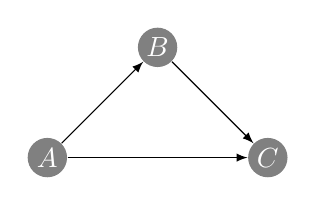
\begin{tikzpicture}[scale=0.7]
  \tikzset{ p/.style={circle,white,fill=gray,inner sep=0pt,minimum size=0.5cm},
  }
  
  \node[p] (A) at (-2, 0) {$A$};
  \node[p] (B) at (0, 2) {$B$};
  \node[p] (C) at (2, 0) {$C$};
  
  \draw[-latex] (A) -- (B) node [midway, above] {};
  \draw[-latex] (B) -- (C) node [midway, above] {};
  \draw[-latex] (A) -- (C) node [midway, above] {};
\end{tikzpicture}
}
\Rightarrow
\parbox[l]{5cm}{

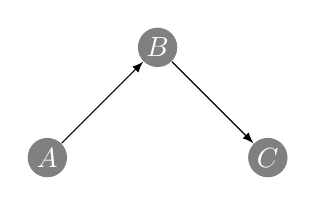
\begin{tikzpicture}[scale=0.7]
  \tikzset{ p/.style={circle,white,fill=gray,inner sep=0pt,minimum size=0.5cm},
  }
  
  \node[p] (A) at (-2, 0) {$A$};
  \node[p] (B) at (0, 2) {$B$};
  \node[p] (C) at (2, 0) {$C$};
  
  \draw[-latex] (A) -- (B) node [midway, above] {};
  \draw[-latex] (B) -- (C) node [midway, above] {};
\end{tikzpicture}
}
\]

Majd bontsuk csoportokra a csúcsokat: az első szinten azon csoportban találhatók
akik kifoka $0$, a másodikon akik kifoka $0$, ha elhagyjuk az első szinten levő
elemeket és így tovább. Majd az első szinten számozzuk meg a pontokat $1$--től
$k_1$--ig, csoporton belül a sorrend nem számit.

A következő szinteken már a pontokat két körben számozzuk:
\begin{itemize}
  \item első körben úgy számozzuk, hogy felsoroljuk mely pontokhoz van élük
  csökkenő sorrendben. E számozásokat lexikografikusan növekvő sorrendbe
  rendezése adja a csoporton belüli sorrendet.
  \item második körben a csoportbeli pontokat számozzuk át, folytatva a korábbi
  csoport számozásától a kapott csoportbeli sorrenddel.
\end{itemize}
 
A kapott számozás szerint csökkenő sorrendbe rakjuk fel a gépekre a munkákat mint
egy listás ütemezés. Ez optimális megoldást ad. 


\subsection{ \texorpdfstring {$ P|in\_tree, p_j=1|C_{max} $} {P|in-tree,pj=1|Cmax} -- Hu algoritmusa}

Ha $D$ precedencia gráf egy $s$ gyökerű $F$--befenyő~\footnote{A befenyő egy
olyan irányított gyökeres fa, aminek az élei a gyökér felé vannak irányítva.},
akkor a szint szerinti ütemezés (gyökértől levő úthossz csökkenő sorrendben)
optimális megoldást ad.
